\documentclass[12pt]{article}
\usepackage[utf8]{inputenc}
\usepackage{amsmath}
\usepackage{graphics}
\author{Carolina Valenzuela Córdova}
\title{\LaTeX}
\date{}
\begin{document}
\title{Reporte Producto 6: Descripción de actividades}
\maketitle{}
  
  En la actividad 6 se modificó el programa realizado en el producto 5, de tal manera que el mismo describiera una trayectoria de tiro parabólico, 
  considerando la fuerza de arrastre o de fricción del objeto con el aire.
A su vez, las ecuaciones de movimiento se modificaron para que se pudiera incluir la fuerza de fricción y que sea graficada correctamente la 
  parábola correspondiente a los parámetros elegidos por el usuario.
  A continuación se presentan los resultados de la práctica con sus respectivas descripciones.\\
  
  Ecuaciones utilizadas para el tiro parabólico sin fricción o fuerza de arrastre:\\
 
 \begin{verbatim}
 Ts = 2*v0*sin*(dt_r)*(1/g)
Ys = v0*v0*sin(dt_r)*sin(dt_r)*(1/(2*g))
Xs = v0*v0*sin(2*dt_r)*(1/g)
  tt(i) = (float(i)*0.01)
  xx(i) = v0x*tt(i) 
  yy(i) = v0y*tt(i) - 0.5*g*tt(i)*tt(i)
 \end{verbatim}


 
  
  
  Como se observa, las ecuaciones aquí son las habituales utilizadas en la mecánica clásica básica, sin considerar la fuerza de fricción entre el objeto lanzado y el aire. 
  Con ellas, el programa nos arroja datos de trayectoria final, como la y máxima, la x máxima o alcance y el tiempo total de vuelo.\\
  
  
  Ecuaciones utilizadas para el tiro parabólico con fricción o fuerza de arrastre:
  


\begin{verbatim}
ft(i+1) = (ft(i)*0.01) + 0.01
  
   vxf(i+1) = vxf(i) + (ax(i)*ft(i+1))
   vyf(i+1) = vyf(i) + (ay(i)*ft(i+1))
   fx(i+1) = fx(i) + (vxf(i)*ft(i+1)) + ((1/2)*ax(i)*ft(i+1)*ft(i+1))
   fy(i+1) = fy(i) + (vyf(i)*ft(i+1)) + ((1/2)*ay(i)*ft(i+1)*ft(i+1))
   ax(i+1) = -(D/m)*(vxf(i))*(vxf(i))
   ay(i+1) = -g - ((D/m)*(vyf(i))*(vyf(i)))
  
\end{verbatim}

  Aquí se debió recurrir a textos de física y páginas de internet como apoyo para articular correctamente las ecuaciones que nos dieran los mismos datos que las anteriores, pero esta vez considerando la fuerza de fricción.\\
  
  Código final del programa:
  \begin{verbatim}
module Cte
implicit none 
real, parameter :: g = 9.81, p =1.1644, pi = 4.0*atan(1.0), CD = 0.47
integer, parameter :: ntps=5000
end module Cte



program Tiro_parabolico
use Cte
implicit none 
real :: dt, x0, y0, v0, v0x, v0y, m, dt_r, D, Xs, Ts, Ys, Xf, Tf, Yf, A, r, ttotal, xsf, ysf, tt, E
real :: vxf(0:ntps), vyf(0:ntps), ax(0:ntps), ay(0:ntps), xx(0:ntps), yy(0:ntps), ft(0:ntps), Vo(0:ntps)


print * , 'Ingreso de datos'
write (*,*) 'Elija una masa para el proyectil'
read *, m
print * , '-------------------------------------'
write (*,*) 'Determine el radio'
read *, r
print * , '-------------------------------------'
write (*,*) 'Proporcione una velocidad inicial'
read *, v0
print * , '-------------------------------------'
write (*,*) 'Ingrese un ángulo inicial para el proyectil'
read *, dt
print * , '-------------------------------------'
write (*,*) 'Determine una posición inicial en el eje x'
read *, x0
print * , '-------------------------------------'
write (*,*) 'Determine una posición inicial en el eje y'
read *, y0
print * , '-------------------------------------'


dt_r =(dt*pi)/180
v0x = v0*cos(dt_r) !velocidad inicial en x
v0y = v0*sin(dt_r) !velocidad inicial en y
A = pi*r*r !area transversal 
D = p*CD*A*0.5 !

 

print * , '-------------------------------------'
print * , '-------------------------------------'
print * , '-------------------------------------'
print * , '-------------------------------------'
print * , '-------------------------------------'


call Tiro_sfriccion(v0, dt_r, v0x, v0y, Xs, Ts, Ys, ttotal, xsf, ysf)
print * , 'Modelo Ideal'
print * , 'Tiempo de vuelo', ttotal, 'segundos'
print * , 'Alcance', xsf, 'metros'
print * , 'Altura máxima', ysf, 'metros'
print * , '-------------------------------------'
print * , '-------------------------------------'
print * , '-------------------------------------'
call Tiro_friccion1(v0, v0x, v0y, ax, ay, Xf, Tf, Yf, x0, y0, vxf, vyf, ft, D, m, Vo)
print * , 'Modelo real'
print * , 'Tiempo de vuelo',Tf ,'segundos'
print * , 'Alcance',Xf ,'metros'
print * , 'Altura máxima',Yf ,'metros'
E=((xsf-Xf)/Xf)*100
print * , 'El error porcentual es', E
end Program Tiro_parabolico



subroutine Tiro_sfriccion(v0, dt_r, v0x, v0y, Xs, Ts, Ys, ttotal, xsf, ysf)
use Cte
implicit none
real, intent(in) :: v0x, v0y, v0, dt_r
real, intent(inout) :: Xs, Ts, Ys, ttotal, xsf, ysf
real, dimension (0:ntps) :: xx, yy, tt
integer :: i

Ts = 2*v0*sin(dt_r)*(1/g)
Ys = v0*v0*sin(dt_r)*sin(dt_r)*(1/(2*g))
Xs = v0*v0*sin(2*dt_r)*(1/g)

open (1, file='tirosinfriccion.dat')
do i=0, ntps, 1
  
  tt(i) = (float(i)*0.01)
  xx(i) = v0x*tt(i) 
  yy(i) = v0y*tt(i) - 0.5*g*tt(i)*tt(i)
write (1,*) xx(i), yy(i)
if (yy(i)<0) exit
end do
close (1)

ttotal =tt(i)
xsf = xx(i)
ysf = maxval(yy, 1, (yy(i)<0))

end subroutine Tiro_sfriccion

subroutine Tiro_friccion1(v0,v0x, v0y, ax, ay, Xf, Tf, Yf, x0, y0, vxf, vyf, ft, D, m, Vo) 
use cte
implicit none
real, intent(in) :: v0, v0x, v0y, x0, y0, D, m
real, intent(inout) :: Xf, Tf, Yf
real, dimension (0:ntps) :: fx, ft, fy, vxf, vyf, ax, ay, Vo
integer :: i
   
   fy = 0
   ft(0)=0
   fx(0)=x0
   fy(0)=y0
   vxf(0)=v0x
   vyf(0)=v0y
   ax(0) = -(D/m)*(v0x)*(v0x)
   ay(0) = -g - ((D/m)*(v0y)*(v0y))

open (2, file='tirofriccion.dat')  
do i = 0, ntps, 1
    

   ft(i+1) = (ft(i)*0.01) + 0.01
  
   vxf(i+1) = vxf(i) + (ax(i)*ft(i+1))
   vyf(i+1) = vyf(i) + (ay(i)*ft(i+1))
   fx(i+1) = fx(i) + (vxf(i)*ft(i+1)) + ((1/2)*ax(i)*ft(i+1)*ft(i+1))
   fy(i+1) = fy(i) + (vyf(i)*ft(i+1)) + ((1/2)*ay(i)*ft(i+1)*ft(i+1))
   ax(i+1) = -(D/m)*(vxf(i))*(vxf(i))
   ay(i+1) = -g - ((D/m)*(vyf(i))*(vyf(i)))
  


write (2, 1001) fx(i), fy(i)
if (fy(i)<0) exit

end do
1001 format (2f10.6)
close (2)

Tf = ft(i) * 10.0
Xf = fx(i+1)
Yf = maxval(fy, 1, (fy(i)<0))
end subroutine Tiro_friccion1
  \end{verbatim}
  

 La estructura del código contempla lo siguiente:
 
Sección de declaración de variables, Sección de declaración de constantes
Subrutina para cálculo de trayectoria con entradas: dt, x0, y0, v0x, v0y, ax, ay; salida: t, x, y ,Subrutina para cálculo de fuerza de arrastre con entrada: m, densidad, A, CD, u0x, v0y ; salida: ax, ay.\\
Se pide que utilizar un formato para escribir salida para los datos (ver ejemplo de formato):
              do i = 1, npts       
              write(1, 10001) x(i), y(i)
       end do 
  1001 format (2f10.6)\\  
 La actividad pide calcular el error al no considerar el arrastre del aire, al lanzar una bola esférica de masa m=0.25kg, y radio R = 0.05m. Hacer un cálculo con y sin arrastre y comparar para ángulos complementarios por arriba y debajo de 45º (por ej. 30º y 60º).
  

 Grafica al menos 3 casos distintos y explica tus resultados desde el punto de vista de la Física.\\
 
  
 \begin{figure}[H]
 \centering
 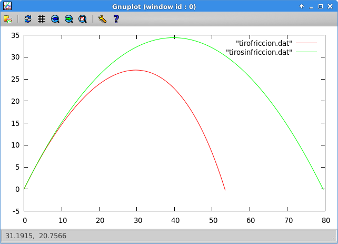
\includegraphics{producto660}
 \caption{Trayectoria a 60 grados con y sin fricción. Error porcentual de 48.4412689 }
 \end{figure}
 
 
 \begin{figure}[H]
 \centering
  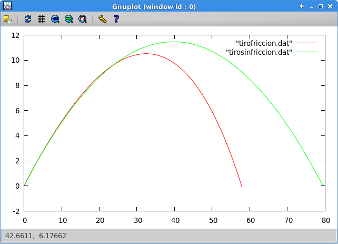
\includegraphics{producto630}
   \caption{Trayectoria a 30 grados con y sin fricción. Error porcentual de 36.9428177 }
  \end{figure}
  
  \begin{figure}[H]
 \centering
 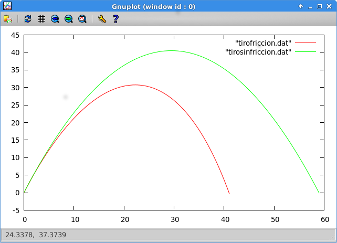
\includegraphics{producto670} 
  \caption{Trayectoria a 70 grados con y sin fricción. Error porcentual de43.4604759}
 \end{figure}
 
 \begin{figure}[H]
 \centering
 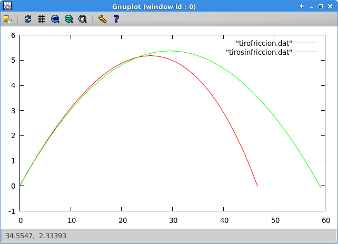
\includegraphics{producto620}
  \caption{Trayectoria a 20 grados con y sin fricción. Error porcentual de26.1744061  }
 \end{figure}
 
 \begin{figure}[H]
 \centering
 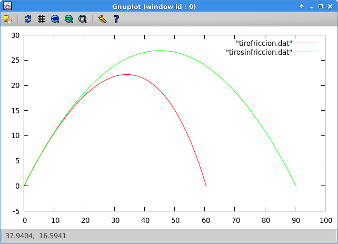
\includegraphics{producto650}
  \caption{Trayectoria a 50 grados con y sin fricción. Error porcentual de 49.0764503 }
 \end{figure}
 
 \begin{figure}[H]
 \centering
 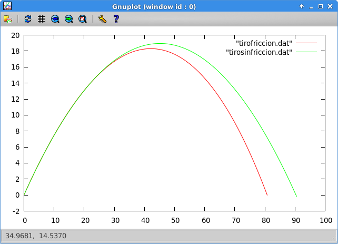
\includegraphics{producto640}
  \caption{Trayectoria a 40 grados con y sin fricción. Error porcentual de 45.0767288  }
 \end{figure}
 
 Como se vio en la explicación proporcionada por el profesor, así como en nuestras clases de mecánica 1, la marcada diferencia entre las dos parábolas arrojadas por el programa está dada por la resistencia del aire, es decir, la fuerza de fricción.
 Tenemos entonces que la aceleración en ambos ejes (x, y), se ve afectada ante la presencia de dicha fuerza, pues hay una evidente pérdida de energía cinética a lo largo de la trayectoria recorrida, debido a la resistencia que se tiene por parte del aire.
 Es así posible que la velocidad en el eje horizontal ya no es constante, y se presenta una deformación en la forma perfectamente simétrica de una parábola convencional sin fricción descrita por la mecánica clásica.
\end{document}